%!TEX root = ../problems.tex
\begin{figure}[h!]
\centering
\begin{minipage}{0.4\textwidth}
\centering
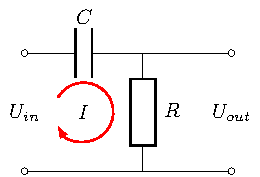
\includegraphics[width=\linewidth]{chem/task4}
\caption{$RC$--контур}
\label{fig:4figsA}
\end{minipage}
\qquad
\begin{minipage}{0.4\textwidth}
\centering
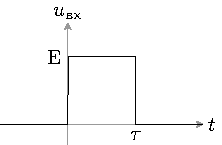
\includegraphics[width=\linewidth]{ris/task4_input}
\caption{Входное напряжение}
\label{fig:4figsB}
\end{minipage}
\end{figure}

\begin{task}
	Определить отклик $u_\out(t)$ $RC$-цепи, изображенной на рисунке, на воздействие прямоугольного импульса длительностью $\tau$. 
	Нарисуйте график отклика. 
	Какова переходная характеристика цепи? 
	При выполнении какого условия будет осуществляться приближённое дифференцирование входной цепи?
	Решить задачу с ненулевыми начальными условиями.
\end{task}
\begin{proof}[\rm{\textbf{Решение}}]
Найдем образ входного импульса преобразованием Лапласа: 
\begin{equation}
	u_\in(t)=E\cdot\H(t)-E\cdot\H(t-\tau)
	\quad\Rightarrow\quad
	u_\in(t)\LT \frac{E}{p}-\frac{E}{p}e^{-p\tau}=
	\frac{E}{p}\qty(1-e^{-p\tau})
\end{equation}
Надо учесть, что в контуре могут быть заданы начальные условия - напряжение на конденсаторе $u_C(0)=u_0$. Его образ $u_C(0) \LT \frac{u_0}{p} $

Обозначим суммарный ток в контуре за $I(p)$. Тогда, так как сумма падений напряжения на каждом элементе равна нулю, получим следующее выражение:
\begin{equation}
	\frac{E}{p}\qty(1-e^{-p\tau})=(R+\frac{1}{pC})I(p)+\frac{u_0}{p}
\end{equation}
Откуда выразим ток $I$:
\begin{equation}
	I(p)=\frac{\frac{E}{p}\qty(1-e^{-p\tau})+u_0/p}{R+\frac{1}{pC}}
\end{equation}
После простых алгебраических преобразований получим:
\begin{equation}
	I(p)=
	\frac{\frac ER }{p+\frac{1}{CR}}-
	\frac{\frac ER e^{-p\tau}}{p+\frac{1}{CR}}-
	\frac{\frac{u_0}R}{p+\frac{1}{CR}}
\end{equation}
Используем свойства преобразования Лапласа:
\begin{gather}
	\frac{\alpha}{p(p+\alpha)}\LT (1-e^{-\alpha t})\H(t)\\
	\frac{1}{(p+\alpha)}\LT e^{-\alpha t}\H(t)\\
	e^{{-p\tau}}F(p) \LT f(t-\tau)\H(t-\tau), \qq{где} F(p) \LT f(t)
\end{gather}
Произведем преобразование:
\begin{gather}
	I(t)=(E-u_0)\frac{\H(t)}{R}\exp{-\frac{t}{CR}}-\frac ER \exp{-\frac{t- \tau	}{CR}}\H(t-\tau )
\end{gather}

Воспользуемся соотношением $u\out=I(t)R$ и окончательно получилим ответ: при воздействии прямоугольным импульсом $u_\in(t)$ амплитуды $E$ и длительностью $\tau$, на выходе получаем
\begin{figure}[h!]
	\centering
	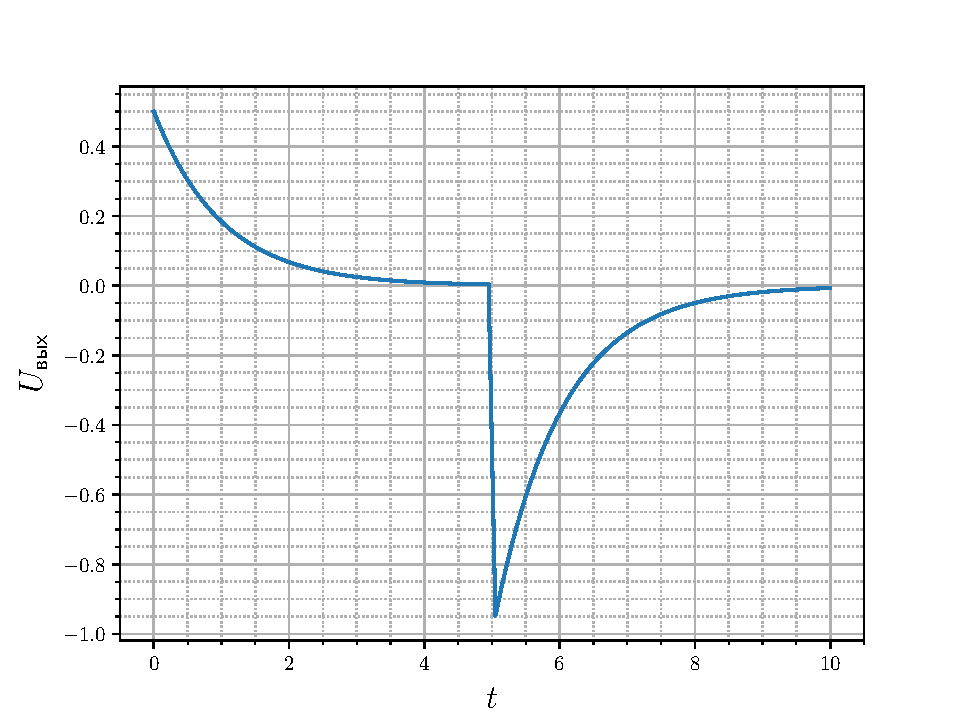
\includegraphics[width=0.7\linewidth]{ris/task4_out}
	\caption{Решение при $E=1, u_0=0.5, \tau=5$}
	\label{fig:4.2}
\end{figure}

\begin{equation}
	u(t)=(E-u_0)\H(t)\exp{-\frac{t}{CR}}-E \exp{-\frac{t- \tau	}{CR}}\H(t-\tau )
\end{equation} 
График решения при $E=1, u_0=0.5, \tau=5$ изображен на рис. \ref{fig:4.2}


\paragraph{Условие дифференцирования.} 
Как нетрудно догадаться,
\begin{equation}
	u_\in=u_C+u_R=\frac{q}{C}+IR
\end{equation}
Продифференцируем это выражение:
\begin{equation}
	\dv{u_\in}{t}=
	\frac{1}{CR}\underbrace{IR}_{u_R\equiv u_\out}+
	\underbrace{\dv{I}{t}R}_{\dv{u_R}{t}}
\end{equation}
Если будет выполнено условие
\begin{equation}
	\abs{\dv{u_R}{t}} \ll \abs{\frac{1}{CR} u_R}
\end{equation}
Тогда будет видно, что цепочка осуществляет дифференцирование:
\begin{equation}
<<<<<<< Updated upstream
	u_\out=RC\dv{u_\in}{t}
=======
	u_\out=CR\dv{u_\in}{t}=\tau_{\text{цепи}}\dv{u_\in}{t}
>>>>>>> Stashed changes
\end{equation}




Выясним смысл неравенства модулей на примере гармонических сигналов. Пусть входное напряжение гармоническое $u_\in=u_0e^{i\omega t}$. Тогда ток в контуре: $I=I_0 e^{i\omega t}$, где $I_0=\frac{u_0}{\frac{1}{i \omega C}+R}$, и неравенство можно переписать (учтем, что $u_C=\frac{I}{i \omega C}=\frac{Ie^{i \omega t}}{i \omega C}$):
\begin{equation}
	\abs{ I_0R \cdot i\omega\cdot e^{i\omega t}}\ll
		\abs{\frac{1}{\tau_\text{цепи}}{I_0}R \cdot e^{i\omega t}}
	\quad \Rightarrow \quad
	\omega \ll {\frac{1}{\tau_\text{цепи}}}
	\quad \Rightarrow \quad
	T \gg \tau_\text{цепи}
\end{equation}
Таким образом, дифференцирование сигнала <<чистое>> для таких частот, период которых много больше постоянной времени цепи. Отсюда следует <<вилка выбора>> дифференцирующей цепочки: если мы будем расширять частотный диапазон <<чистого>> дифференцирования уменьшением постоянной времени, то амплитуда на выходе цепочки будет падать, и наоборот.


\end{proof}